

\tikzset{every picture/.style={line width=0.75pt}} %set default line width to 0.75pt        

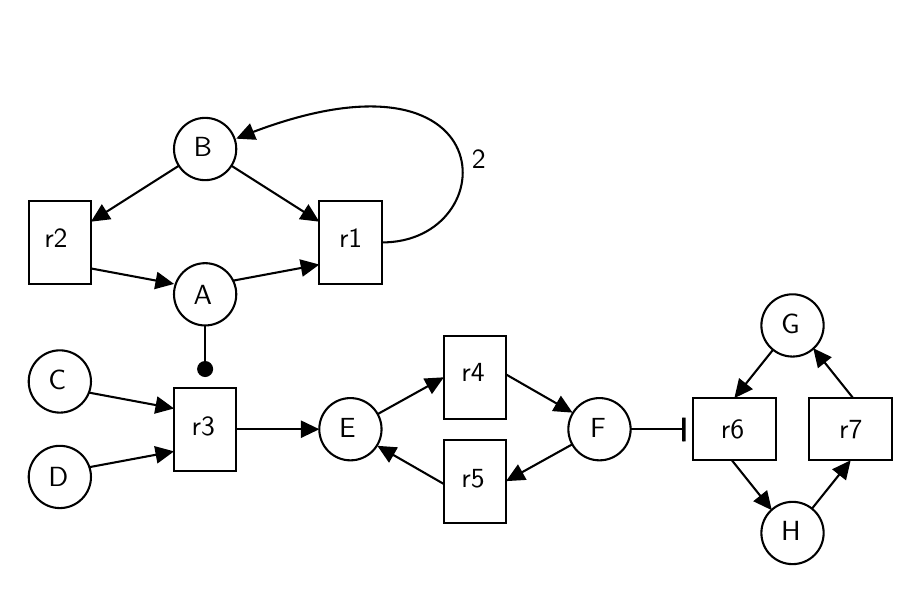
\begin{tikzpicture}[x=0.75pt,y=0.75pt,yscale=-1,xscale=1]
%uncomment if require: \path (0,300); %set diagram left start at 0, and has height of 300

%Straight Lines [id:da3576438741903769] 
\draw    (388,210) -- (414.13,177.34) ;
\draw [shift={(416,175)}, rotate = 488.66] [fill={rgb, 255:red, 0; green, 0; blue, 0 }  ][line width=0.08]  [draw opacity=0] (8.93,-4.29) -- (0,0) -- (8.93,4.29) -- cycle    ;
%Straight Lines [id:da5206527388854192] 
\draw    (350,164) -- (376.13,196.66) ;
\draw [shift={(378,199)}, rotate = 231.34] [fill={rgb, 255:red, 0; green, 0; blue, 0 }  ][line width=0.08]  [draw opacity=0] (8.93,-4.29) -- (0,0) -- (8.93,4.29) -- cycle    ;
%Straight Lines [id:da9664135693242828] 
\draw    (388,110) -- (361.87,142.66) ;
\draw [shift={(360,145)}, rotate = 308.65999999999997] [fill={rgb, 255:red, 0; green, 0; blue, 0 }  ][line width=0.08]  [draw opacity=0] (8.93,-4.29) -- (0,0) -- (8.93,4.29) -- cycle    ;
%Straight Lines [id:da3150124855239005] 
\draw    (426,156) -- (399.87,123.34) ;
\draw [shift={(398,121)}, rotate = 411.34000000000003] [fill={rgb, 255:red, 0; green, 0; blue, 0 }  ][line width=0.08]  [draw opacity=0] (8.93,-4.29) -- (0,0) -- (8.93,4.29) -- cycle    ;
%Straight Lines [id:da2531638133399581] 
\draw    (295,160) -- (335,160) ;
%Straight Lines [id:da7978054588524539] 
\draw    (110,160) -- (157,160) ;
\draw [shift={(160,160)}, rotate = 180] [fill={rgb, 255:red, 0; green, 0; blue, 0 }  ][line width=0.08]  [draw opacity=0] (8.93,-4.29) -- (0,0) -- (8.93,4.29) -- cycle    ;
%Straight Lines [id:da5621074466789615] 
\draw    (235,125) -- (279.4,150.51) ;
\draw [shift={(282,152)}, rotate = 209.88] [fill={rgb, 255:red, 0; green, 0; blue, 0 }  ][line width=0.08]  [draw opacity=0] (8.93,-4.29) -- (0,0) -- (8.93,4.29) -- cycle    ;
%Straight Lines [id:da9432384230142636] 
\draw    (235,195) -- (190.6,169.49) ;
\draw [shift={(188,168)}, rotate = 389.88] [fill={rgb, 255:red, 0; green, 0; blue, 0 }  ][line width=0.08]  [draw opacity=0] (8.93,-4.29) -- (0,0) -- (8.93,4.29) -- cycle    ;
%Straight Lines [id:da2732887752012232] 
\draw    (295,160) -- (252.62,183.54) ;
\draw [shift={(250,185)}, rotate = 330.95] [fill={rgb, 255:red, 0; green, 0; blue, 0 }  ][line width=0.08]  [draw opacity=0] (8.93,-4.29) -- (0,0) -- (8.93,4.29) -- cycle    ;
%Straight Lines [id:da8361705783456022] 
\draw    (175,160) -- (217.38,136.46) ;
\draw [shift={(220,135)}, rotate = 510.95] [fill={rgb, 255:red, 0; green, 0; blue, 0 }  ][line width=0.08]  [draw opacity=0] (8.93,-4.29) -- (0,0) -- (8.93,4.29) -- cycle    ;
%Straight Lines [id:da26704871020062715] 
\draw    (110,90) -- (157.05,81.23) ;
\draw [shift={(160,80.68)}, rotate = 529.44] [fill={rgb, 255:red, 0; green, 0; blue, 0 }  ][line width=0.08]  [draw opacity=0] (8.93,-4.29) -- (0,0) -- (8.93,4.29) -- cycle    ;
%Straight Lines [id:da4846937260313433] 
\draw    (40,80.68) -- (87.05,89.45) ;
\draw [shift={(90,90)}, rotate = 190.56] [fill={rgb, 255:red, 0; green, 0; blue, 0 }  ][line width=0.08]  [draw opacity=0] (8.93,-4.29) -- (0,0) -- (8.93,4.29) -- cycle    ;
%Straight Lines [id:da271105016276878] 
\draw    (105,25) -- (157.47,58.39) ;
\draw [shift={(160,60)}, rotate = 212.47] [fill={rgb, 255:red, 0; green, 0; blue, 0 }  ][line width=0.08]  [draw opacity=0] (8.93,-4.29) -- (0,0) -- (8.93,4.29) -- cycle    ;
%Shape: Rectangle [id:dp9228181661849988] 
\draw  [fill={rgb, 255:red, 255; green, 255; blue, 255 }  ,fill opacity=1 ] (20,50) -- (50,50) -- (50,90) -- (20,90) -- cycle ;
%Straight Lines [id:da06467494297119436] 
\draw    (105,25) -- (52.53,58.39) ;
\draw [shift={(50,60)}, rotate = 327.53] [fill={rgb, 255:red, 0; green, 0; blue, 0 }  ][line width=0.08]  [draw opacity=0] (8.93,-4.29) -- (0,0) -- (8.93,4.29) -- cycle    ;
%Shape: Circle [id:dp49236484975772] 
\draw  [fill={rgb, 255:red, 255; green, 255; blue, 255 }  ,fill opacity=1 ] (90,25) .. controls (90,16.72) and (96.72,10) .. (105,10) .. controls (113.28,10) and (120,16.72) .. (120,25) .. controls (120,33.28) and (113.28,40) .. (105,40) .. controls (96.72,40) and (90,33.28) .. (90,25) -- cycle ;
%Shape: Rectangle [id:dp3146550401206405] 
\draw  [fill={rgb, 255:red, 255; green, 255; blue, 255 }  ,fill opacity=1 ] (160,50) -- (190,50) -- (190,90) -- (160,90) -- cycle ;
%Curve Lines [id:da9984566963389516] 
\draw    (190,70) .. controls (250.06,70.4) and (250.75,-32.96) .. (121.95,19.2) ;
\draw [shift={(120,20)}, rotate = 337.56] [fill={rgb, 255:red, 0; green, 0; blue, 0 }  ][line width=0.08]  [draw opacity=0] (8.93,-4.29) -- (0,0) -- (8.93,4.29) -- cycle    ;
%Shape: Circle [id:dp09345090103745823] 
\draw  [fill={rgb, 255:red, 255; green, 255; blue, 255 }  ,fill opacity=1 ] (90,95) .. controls (90,86.72) and (96.72,80) .. (105,80) .. controls (113.28,80) and (120,86.72) .. (120,95) .. controls (120,103.28) and (113.28,110) .. (105,110) .. controls (96.72,110) and (90,103.28) .. (90,95) -- cycle ;
%Straight Lines [id:da5223576478149881] 
\draw    (105,110) -- (105,131) ;
\draw [shift={(105,131)}, rotate = 90] [color={rgb, 255:red, 0; green, 0; blue, 0 }  ][fill={rgb, 255:red, 0; green, 0; blue, 0 }  ][line width=0.75]      (0, 0) circle [x radius= 3.35, y radius= 3.35]   ;
%Shape: Rectangle [id:dp25364205729175127] 
\draw  [fill={rgb, 255:red, 255; green, 255; blue, 255 }  ,fill opacity=1 ] (90,140) -- (120,140) -- (120,180) -- (90,180) -- cycle ;
%Straight Lines [id:da8084682726089965] 
\draw    (40,140.68) -- (87.05,149.45) ;
\draw [shift={(90,150)}, rotate = 190.56] [fill={rgb, 255:red, 0; green, 0; blue, 0 }  ][line width=0.08]  [draw opacity=0] (8.93,-4.29) -- (0,0) -- (8.93,4.29) -- cycle    ;
%Straight Lines [id:da8278541197200837] 
\draw    (40,180) -- (87.05,171.23) ;
\draw [shift={(90,170.68)}, rotate = 529.44] [fill={rgb, 255:red, 0; green, 0; blue, 0 }  ][line width=0.08]  [draw opacity=0] (8.93,-4.29) -- (0,0) -- (8.93,4.29) -- cycle    ;
%Shape: Circle [id:dp5697702501712039] 
\draw  [fill={rgb, 255:red, 255; green, 255; blue, 255 }  ,fill opacity=1 ] (20,137) .. controls (20,128.72) and (26.72,122) .. (35,122) .. controls (43.28,122) and (50,128.72) .. (50,137) .. controls (50,145.28) and (43.28,152) .. (35,152) .. controls (26.72,152) and (20,145.28) .. (20,137) -- cycle ;
%Shape: Circle [id:dp027027959729662543] 
\draw  [fill={rgb, 255:red, 255; green, 255; blue, 255 }  ,fill opacity=1 ] (20,183) .. controls (20,174.72) and (26.72,168) .. (35,168) .. controls (43.28,168) and (50,174.72) .. (50,183) .. controls (50,191.28) and (43.28,198) .. (35,198) .. controls (26.72,198) and (20,191.28) .. (20,183) -- cycle ;
%Shape: Circle [id:dp7929646959402241] 
\draw  [fill={rgb, 255:red, 255; green, 255; blue, 255 }  ,fill opacity=1 ] (160,160) .. controls (160,151.72) and (166.72,145) .. (175,145) .. controls (183.28,145) and (190,151.72) .. (190,160) .. controls (190,168.28) and (183.28,175) .. (175,175) .. controls (166.72,175) and (160,168.28) .. (160,160) -- cycle ;
%Shape: Rectangle [id:dp05655391624383377] 
\draw  [fill={rgb, 255:red, 255; green, 255; blue, 255 }  ,fill opacity=1 ] (220,115) -- (250,115) -- (250,155) -- (220,155) -- cycle ;
%Shape: Rectangle [id:dp05796590340987029] 
\draw  [fill={rgb, 255:red, 255; green, 255; blue, 255 }  ,fill opacity=1 ] (220,165) -- (250,165) -- (250,205) -- (220,205) -- cycle ;
%Shape: Circle [id:dp13273124949760895] 
\draw  [fill={rgb, 255:red, 255; green, 255; blue, 255 }  ,fill opacity=1 ] (280,160) .. controls (280,151.72) and (286.72,145) .. (295,145) .. controls (303.28,145) and (310,151.72) .. (310,160) .. controls (310,168.28) and (303.28,175) .. (295,175) .. controls (286.72,175) and (280,168.28) .. (280,160) -- cycle ;
%Straight Lines [id:da9347007050049654] 
\draw    (335.29,154.43) -- (335.26,165.81) ;
%Straight Lines [id:da20553639689795267] 
\draw    (336,154.43) -- (335.97,165.81) ;
%Shape: Rectangle [id:dp30165349356224813] 
\draw  [fill={rgb, 255:red, 255; green, 255; blue, 255 }  ,fill opacity=1 ] (380,145) -- (380,175) -- (340,175) -- (340,145) -- cycle ;
%Shape: Rectangle [id:dp05448702121100979] 
\draw  [fill={rgb, 255:red, 255; green, 255; blue, 255 }  ,fill opacity=1 ] (436,145) -- (436,175) -- (396,175) -- (396,145) -- cycle ;
%Shape: Circle [id:dp37659499504730287] 
\draw  [fill={rgb, 255:red, 255; green, 255; blue, 255 }  ,fill opacity=1 ] (373,110) .. controls (373,101.72) and (379.72,95) .. (388,95) .. controls (396.28,95) and (403,101.72) .. (403,110) .. controls (403,118.28) and (396.28,125) .. (388,125) .. controls (379.72,125) and (373,118.28) .. (373,110) -- cycle ;
%Shape: Circle [id:dp13055596917815526] 
\draw  [fill={rgb, 255:red, 255; green, 255; blue, 255 }  ,fill opacity=1 ] (373,210) .. controls (373,201.72) and (379.72,195) .. (388,195) .. controls (396.28,195) and (403,201.72) .. (403,210) .. controls (403,218.28) and (396.28,225) .. (388,225) .. controls (379.72,225) and (373,218.28) .. (373,210) -- cycle ;

% Text Node
\draw (26,62) node [anchor=north west][inner sep=0.75pt]   [align=left] {$\mathsf{r2}$};
% Text Node
\draw (168,62) node [anchor=north west][inner sep=0.75pt]   [align=left] {$\mathsf{r1}$};
% Text Node
\draw (97,153) node [anchor=north west][inner sep=0.75pt]   [align=left] {$\mathsf{r3}$};
% Text Node
\draw (227,127) node [anchor=north west][inner sep=0.75pt]   [align=left] {$\mathsf{r4}$};
% Text Node
\draw (227,178) node [anchor=north west][inner sep=0.75pt]   [align=left] {$\mathsf{r5}$};
% Text Node
\draw (352,154) node [anchor=north west][inner sep=0.75pt]   [align=left] {$\mathsf{r6}$};
% Text Node
\draw (409,154) node [anchor=north west][inner sep=0.75pt]   [align=left] {$\mathsf{r7}$};

% Text Node
\draw (98,18) node [anchor=north west][inner sep=0.75pt]   [align=left] {$\mathsf{B}$};
% Text Node
\draw (98,89) node [anchor=north west][inner sep=0.75pt]   [align=left] {$\mathsf{A}$};
% Text Node
\draw (28,130) node [anchor=north west][inner sep=0.75pt]   [align=left] {$\mathsf{C}$};
% Text Node
\draw (28,177) node [anchor=north west][inner sep=0.75pt]   [align=left] {$\mathsf{D}$};
% Text Node
\draw (168,153) node [anchor=north west][inner sep=0.75pt]   [align=left] {$\mathsf{E}$};
% Text Node
\draw (289,153) node [anchor=north west][inner sep=0.75pt]   [align=left] {$\mathsf{F}$};
% Text Node
\draw (381,103) node [anchor=north west][inner sep=0.75pt]   [align=left] {$\mathsf{G}$};
% Text Node
\draw (381,203) node [anchor=north west][inner sep=0.75pt]   [align=left] {$\mathsf{H}$};
% Text Node
\draw (232,24) node [anchor=north west][inner sep=0.75pt]   [align=left] {$\mathsf{2}$};


\end{tikzpicture}